%% This is file `elsarticle-template-1-num.tex',
%%
%% Copyright 2009 Elsevier Ltd
%%
%% This file is part of the 'Elsarticle Bundle'.
%% ---------------------------------------------
%%
%% It may be distributed under the conditions of the LaTeX Project Public
%% License, either version 1.2 of this license or (at your option) any
%% later version.  The latest version of this license is in
%%    http://www.latex-project.org/lppl.txt
%% and version 1.2 or later is part of all distributions of LaTeX
%% version 1999/12/01 or later.
%%
%% Template article for Elsevier's document class `elsarticle'
%% with numbered style bibliographic references
%%
%% $Id: elsarticle-template-1-num.tex 149 2009-10-08 05:01:15Z rishi $
%% $URL: http://lenova.river-valley.com/svn/elsbst/trunk/elsarticle-template-1-num.tex $
%%
%\documentclass[preprint,12pt]{elsarticle}

%% Use the option review to obtain double line spacing
%% \documentclass[preprint,review,12pt]{elsarticle}

%% Use the options 1p,twocolumn; 3p; 3p,twocolumn; 5p; or 5p,twocolumn
%% for a journal layout:
 \documentclass[final,review,3p,times,12pt]{elsarticle}
%% \documentclass[final,1p,times,twocolumn]{elsarticle}
%% \documentclass[final,3p,times]{elsarticle}
%% \documentclass[final,3p,times,twocolumn]{elsarticle}
%% \documentclass[final,5p,times]{elsarticle}
%% \documentclass[final,5p,times,twocolumn]{elsarticle}

%% The graphicx package provides the includegraphics command.
\usepackage{graphicx}
%% The amssymb package provides various useful mathematical symbols
\usepackage{amssymb}
%% The amsthm package provides extended theorem environments
%% \usepackage{amsthm}

%% The lineno packages adds line numbers. Start line numbering with
%% \begin{linenumbers}, end it with \end{linenumbers}. Or switch it on
%% for the whole article with \linenumbers after \end{frontmatter}.
%\usepackage{lineno}

%% natbib.sty is loaded by default. However, natbib options can be
%% provided with \biboptions{...} command. Following options are
%% valid:

%%   round  -  round parentheses are used (default)
%%   square -  square brackets are used   [option]
%%   curly  -  curly braces are used      {option}
%%   angle  -  angle brackets are used    <option>
%%   semicolon  -  multiple citations separated by semi-colon
%%   colon  - same as semicolon, an earlier confusion
%%   comma  -  separated by comma
%%   numbers-  selects numerical citations
%%   super  -  numerical citations as superscripts
%%   sort   -  sorts multiple citations according to order in ref. list
%%   sort&compress   -  like sort, but also compresses numerical citations
%%   compress - compresses without sorting
%%
%% \biboptions{comma,round}

% \biboptions{}

\journal{Focus on Quantum Coherent Feedback and Reservoir Engineering}

\pdfoutput=1
\usepackage[latin1]{inputenc}
\usepackage{amsmath}
\usepackage{amssymb}
\usepackage{color}
\usepackage{citesort}

\usepackage{mathtools}
\usepackage{float}
\usepackage[T1]{fontenc}

\def\ket#1{|#1\rangle}
\def\e#1{ e^{#1}}
\def\bra#1{\langle#1|}
\def\av#1{\langle#1\rangle}

\def\tder#1{\frac{d#1}{dt}}
\def\eps{\varepsilon}
\def\nup{\nu^\prime}

\def\aop{\hat{a}}
\def\adop{\hat{a}^\dagger}
\def\awop{\tilde{a}}
\def\awdop{\tilde{a}^\dagger}
\def\bop{\hat{b}}
\def\bdop{\hat{b}^\dagger}
\def\bwop{\tilde{b}}
\def\bwdop{\tilde{b}^\dagger}
\def\cop{\hat{c}}
\def\cwop{\tilde{c}}
\def\cwdop{\tilde{c}^\dagger}
\def\Xop{\hat{X}}
\def\thetap{\theta^\prime}
\def\Xwop{\hat{\tilde{X}}}
\def\Hop{\hat{H}}
\def\Bop{\hat{B}}
\def\Bdop{\hat{B}^\dagger}
\def\nuop{\hat{\nu}}
\def\xiop{\hat{\xi}}
\def\xidop{\hat{\xi}^\dagger}
\def\xiwop{\tilde{\xi}}
\def\xiwdop{\tilde{\xi}^\dagger}
\def\thetap{{\theta^\prime}}
\def\mnu{{-\nu}}
\def\sm{{-}}

\def\nn{\nonumber}

\newcommand{\lsz}{\left[}
\newcommand{\rsz}{\right]}
\newcommand{\lk}{\left(}
\newcommand{\rk}{\right)}
\newcommand{\lka}{\left\{}
\newcommand{\rka}{\right\}}
\newcommand{\labs}{\left|}
\newcommand{\rabs}{\right|}
\pdfminorversion=4

\usepackage{hyperref}
\def\refeq#1{{\hyperref[#1]{(\ref*{#1})}}}
\def\reffig#1{{\hyperref[#1]{FIG. \ref*{#1}}}}
\def\refsec#1{{\hyperref[#1]{SEC. \ref*{#1}}}}
\def\refno#1{{\hyperref[#1]{\ref*{#1}}}}
\def\dul#1{\underline{\underline{#1}}}
\def\ul#1{\underline{#1}}
\def\frvecop#1{\hat{\tilde{\underline{#1}}}}
\def\frmat#1{\tilde{\dul{#1}}}
\def\myeq#1{\stackrel{\mathclap{\tiny\mbox{#1}}}{=}}
\def\frop#1{\hat{\tilde{#1}}}
\def\av#1{\langle#1\rangle}

\newcommand{\gguide}{{\it NDPA paper}}
%Uncomment next line if AMS fonts required
%\usepackage{iopams}  
\begin{document}

\begin{frontmatter}

\title{Enhancement of EPR-type entanglement in an NDPA with coherent time-delayed feedback}

\author{Nikolett N\'emet and Scott Parkins}

\address{The Dodd-Walls Centre for Photonic and Quantum Technologies,\\
Department of Physics, University of Auckland, New Zealand}
\ead{nnem614@aucklanduni.ac.nz}
\begin{abstract}
This paper presents an analysis on the effects of coherent time-delayed feedback of the down-converted fields in a Nondegenerate Parametric Amplifier. We observe enhanced Einstein-Podolsky-Rosen type of entanglement between the two modes at a given driving strength. Increased correlation can be shown both on resonance and at shifted frequencies due to the finite time-delay in the feedback loops.
\end{abstract}
\end{frontmatter}
%Uncomment for PACS numbers title message
%\pacs{00.00, 20.00, 42.10}
% Keywords required only for MST, PB, PMB, PM, JOA, JOB? 
%\vspace{2pc}
%\noindent{\it Keywords}: Article preparation, IOP journals
% Uncomment for Submitted to journal title message
%\submitto{\JPA}
% Comment out if separate title page not required
%\linenumbers

\section{Introduction}
Quantum information theory is a very topical research field both from a fundamental and applied perspective. Most investigations target discreet variables, where due to the orthogonality of the applied basis completely unitary transformations are available in principle. However, loss of information and decoherence due to the surrounding environment results in an adverse probabilistic nature of the originally deterministic manipulations e.g. preparation of an entangled state. On the other hand using continuous variables, entangled states are obtained in nonlinear optical processes, although at the expense of reduced "quality" of entanglement \cite{Braunstein2005}.

In 1935 Einstein, Podolsky and Rosen published there well-known paper about non-locality \cite{Einstein1935}. In this paper they discussed the strong correlations between the continuous degrees of freedom of spatially separate particles. The question of non-locality shifted towards discreet variables, but strong correlations of continuous variables remained a question. 

\begin{figure}[h!]
\centering
%\vglue -.2 cm
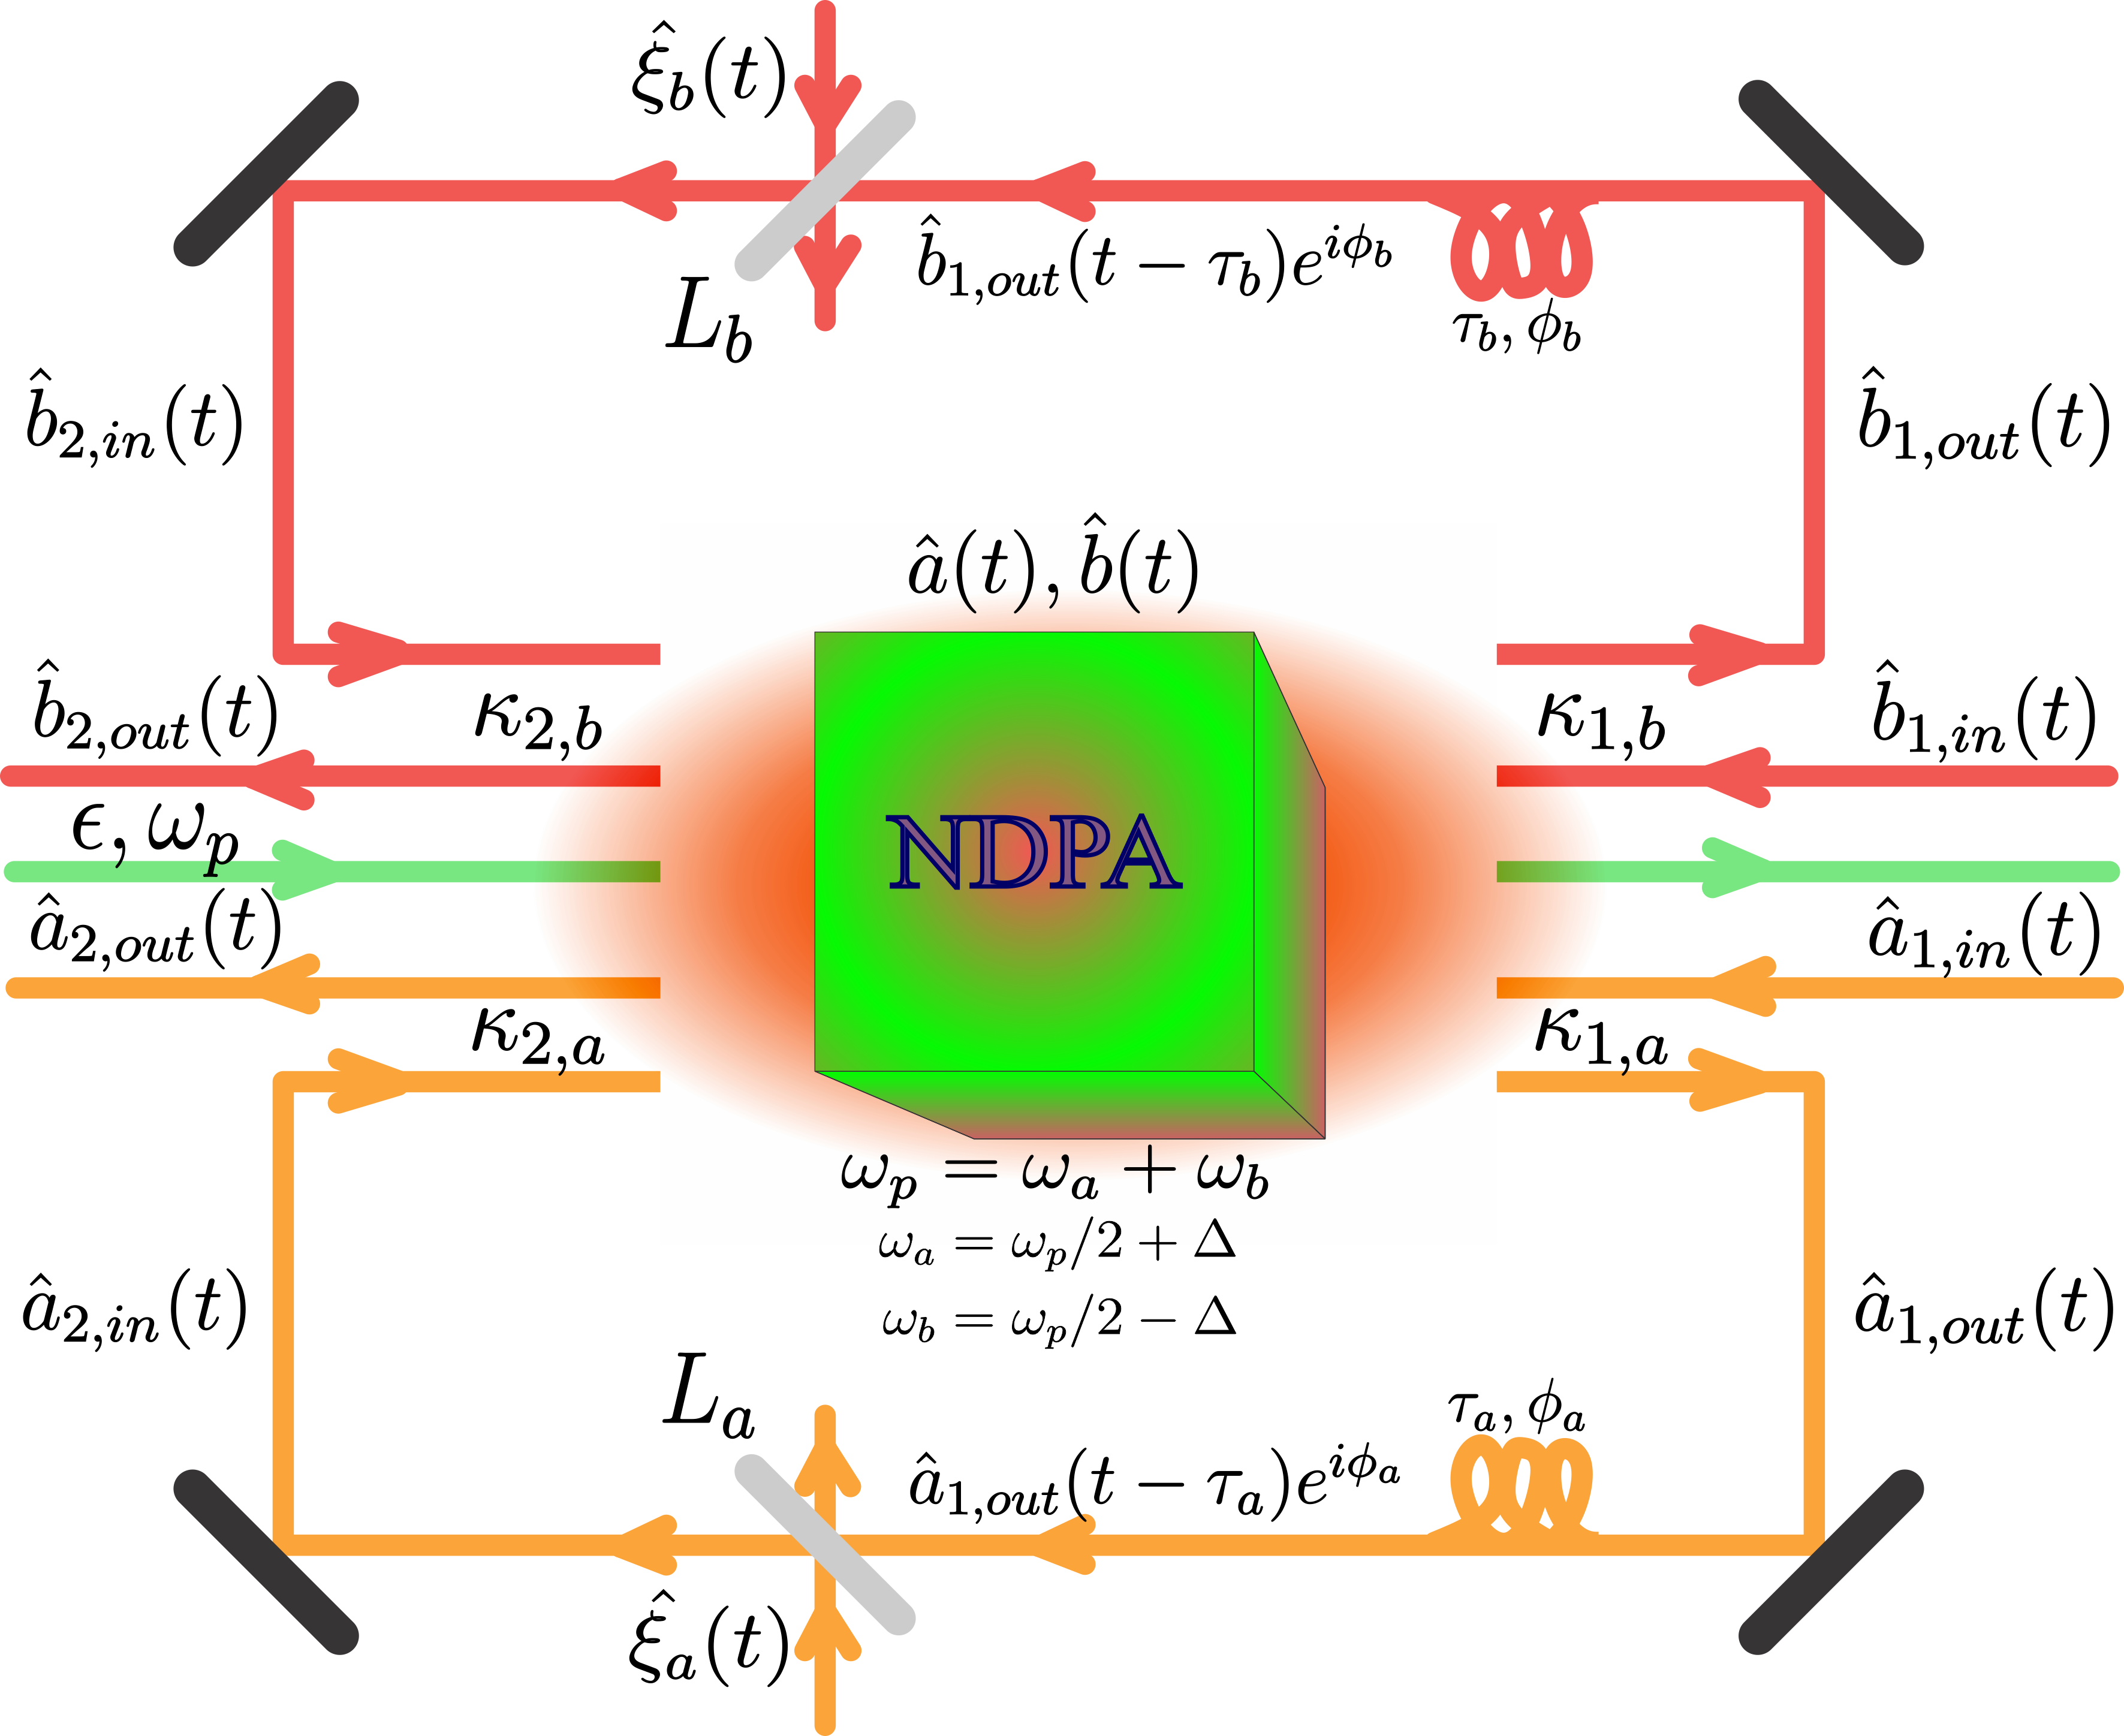
\includegraphics[width=.9\textwidth]{figure1.png}
\vglue -1 cm
\textit{\textbf{\caption{\linespread{1}\small{Schematic setup. The nonlinear crystal performing parametric down-conversion on the incoming photons is placed in a cavity. The output fields on the right hand side is directly coupled back into the input channels of the other side without performing any measurement. The longer length of the loops support a finite time-delay in the feedback loop ($\tau_{a,b}$) and phase shift ($\phi_{a,b}$). Losses are also incorporated in the feedback loop with a beam splitter model.}}\label{fig:setup}}}
%\vglue -.3 cm
\end{figure}

One of the first proposed setup, where such a continuous variable entanglement can be generated was the Non-degenerate Parametric Amplifier (NDPA) \cite{Collett1987,Drummond1990}. A crystal with $\chi^{(2)}$ nonlinearity, which performs parametric down-conversion of the pumping mode into two separate modes, is placed in a cavity. Measuring the  quadratures of the two down-converted modes showed strong correlation or anti-correlation depending on the quadrature angle \cite{Ou1992}.

In order to overcome the intrinsic limitations in the entangling performance of NDPA, cascaded \cite{He2007,Shi2016a} and feedback setups (depicted in \reffig{fig:setup} $\left. b\right)$ \cite{Yan2011,Zhou2015}) were proposed. The latter has been already proven beneficial in entangling discreet variables \cite{Hein2015} and enhancement of squeezing in the Degenerate Parametric Amplifier (DPA) \cite{Gough2009, Iida2012, Nemet2016, Kraft2016}. In case of the NDPA setup, enhanced entanglement \cite{Yan2011,Zhou2015} as well as broadened spectra of two-mode squeezing \cite{Yan2011,Zhou2015} was obtained.

In this paper we propose a time-delayed coherent feedback setup depicted in \reffig{fig:setup} $\left. c\right)$, where the output fields of one side are directly coupled back into the input channels of the other side. The length of the feedback loops support generally different finite time-delays $\tau_a, \tau_b$. In the most general case the mirrors of the cavity have different transmission rate on each side $(1,2)$ for each down-converted mode ($\kappa_{1/2,a/b}$). The phase shifts picked up as a result of the frequency difference, reflections and other processes are included in the phase factors $\phi_{a,b}$ separately for each mode.

\section{EPR-type entanglement in NDPA}
Detection of EPR-type entanglement in NDPA is based on the consequent noise reduction of the combined quadrature of the two down-converted modes \cite{Collett1987,Drummond1990}. Measuring this reduced uncertainty requires the observation of a two-mode squeezing spectrum of the generalized quadrature \cite{Caves1985,Schumaker1985} in a heterodyne (in case of two non-overlapping modes) or coupled homodyne scheme (for frequency-degenerates modes with orthogonal polarization) \cite{Drummond1990}.

Let us consider the quadratures of the two down-converted modes $\aop$ and $\bop$ as
\begin{align*}
\hat{X}_{a,\thetap_a}&=\frac{1}{2}\lk\aop e^{-i\thetap_a/2}+\adop e^{i\thetap_a/2}\rk&\hat{X}_{b,\thetap_b}&=\frac{1}{2}\lk\bop e^{-i\thetap_b/2}+\bdop e^{i\thetap_b/2}\rk\\
\hat{Y}_{a,\thetap_a}&=\frac{1}{2i}\lk\aop e^{-i\thetap_a/2}-\adop e^{i\thetap_a/2}\rk&
\hat{Y}_{b,\thetap_b}&=\frac{1}{2i}\lk\bop e^{-i\thetap_b/2}-\bdop e^{i\thetap_b/2}\rk
\end{align*}
and the generalized quadrature for two-mode squeezing is:
\begin{align}
\hat{X}_\thetap^G=\hat{X}_{a,\thetap_a}+\hat{X}_{b,\thetap_b}\\
\hat{Y}_\thetap^G=\hat{Y}_{a,\thetap_a}-\hat{Y}_{b,\thetap_b}
\end{align}
Two-mode squeezing occurs, when the sum of the normal-ordered variance of $\hat{X}_\thetap^G$ and $\hat{Y}_\thetap^G$ is less than $0$.
\begin{align}
\left\langle\lk\Delta\hat{X}_\thetap^G\rk^2\right\rangle+\left\langle\lk\Delta\hat{Y}_\thetap^G\rk^2\right\rangle<0\\
\left\langle\lk\Delta\hat{O}\rk^2\right\rangle=\left\langle\hat{O}^2\right\rangle-\left\langle\hat{O}\right\rangle^2
\end{align}
Let us introduce the frequency-dependent operators as:
\begin{align}
\hat{\tilde{O}}(\nu)=\frac{1}{\sqrt{2\pi}}\int_{-\infty}^\infty e^{i\nu t}\hat{O}(t)dt
\end{align}
In a one-sided cavity without feedback, where the down-converted modes have the same frequency but orthogonal polarization this expression has the following form \cite{Collett1987}:
\begin{align}
\chi_\thetap^\text{no fb}(\nu)&=\int_{-\infty}^\infty\lsz\left\langle\lk\Delta\hat{\tilde{X}}_\thetap^G\rk^2(\nu,\nup)\right\rangle+\left\langle\lk\Delta\hat{\tilde{Y}}_\thetap^G\rk^2(\nu,\nup)\right\rangle\rsz d\nup=\\
&=\lka 1+4|\epsilon|\kappa\lsz\frac{\cos^2{\lk\frac{\theta}{2}-\frac{\thetap_a+\thetap_b}{4}\rk}}{\lk\kappa-|\epsilon|\rk^2+\nu^2}-\frac{\sin^2{\lk\frac{\theta}{2}-\frac{\thetap_a+\thetap_b}{4}\rk}}{\lk\kappa+|\epsilon|\rk^2+\nu^2}\rsz\rka
\end{align}
In case of the phase quadrature $\frac{\thetap}{2}=\frac{\theta}{2}-\frac{\thetap_a+\thetap_b}{4}=\frac{\pi}{2}$ this expression simplifies to the following
\begin{align}
\chi_\pi^\text{no fb}(\nu)=1-\frac{4|\epsilon|\kappa}{\lk\kappa+|\epsilon|\rk^2+\nu^2}
\end{align}
which vanishes on threshold ($|\epsilon|=\kappa$), on resonance providing perfect two-mode squeezing. This means in principle complete noiseless correlation between the measured values of the two down-converted quadratures.

\section{Theoretical model}
Generally the equation of motion of system operators have the following form, when memory-effects are present \cite{Whalen2016}:
\begin{align}
\frac{d}{dt}\hat{\underline{a}}(t) = \frac{i}{\hbar}\lsz\Hop_S, \hat{\underline{a}}(t)\rsz - 
\int_0^t\dul{f}(t-t^\prime)\hat{\underline{a}}(t^\prime) - 
i\left(\underline{\Omega}(t)+\hat{\underline{B}}(t)\right)
\end{align}
where $\Hop_S$ represents the Hamiltonian of the closed system, $\dul{f}(t)$ is the dissipation kernel, a coherent driving can be included as $\underline{\Omega}(t)$ and the input field as an operator is incorporated as $\underline{\Bop}(t)$. Where the dissipation kernel and the input field are related via the spectral density $\dul{J}_{\alpha}(\omega)$ of environment labeled $\alpha$:
\begin{align}
f_{jk}(t_{1}-t_{2})=\lsz\Bop_j(t_1),\Bdop_k(t_2)\rsz=\sum_\alpha\int_{-\infty}^\infty J_{\alpha jk}(\omega)e^{-i\omega (t_{1}-t_{2})}d\omega
\end{align}

\section{Without time-delay}
\section{With time-delay}
\begin{figure}[h!]
\centering
%\vglue -.2 cm
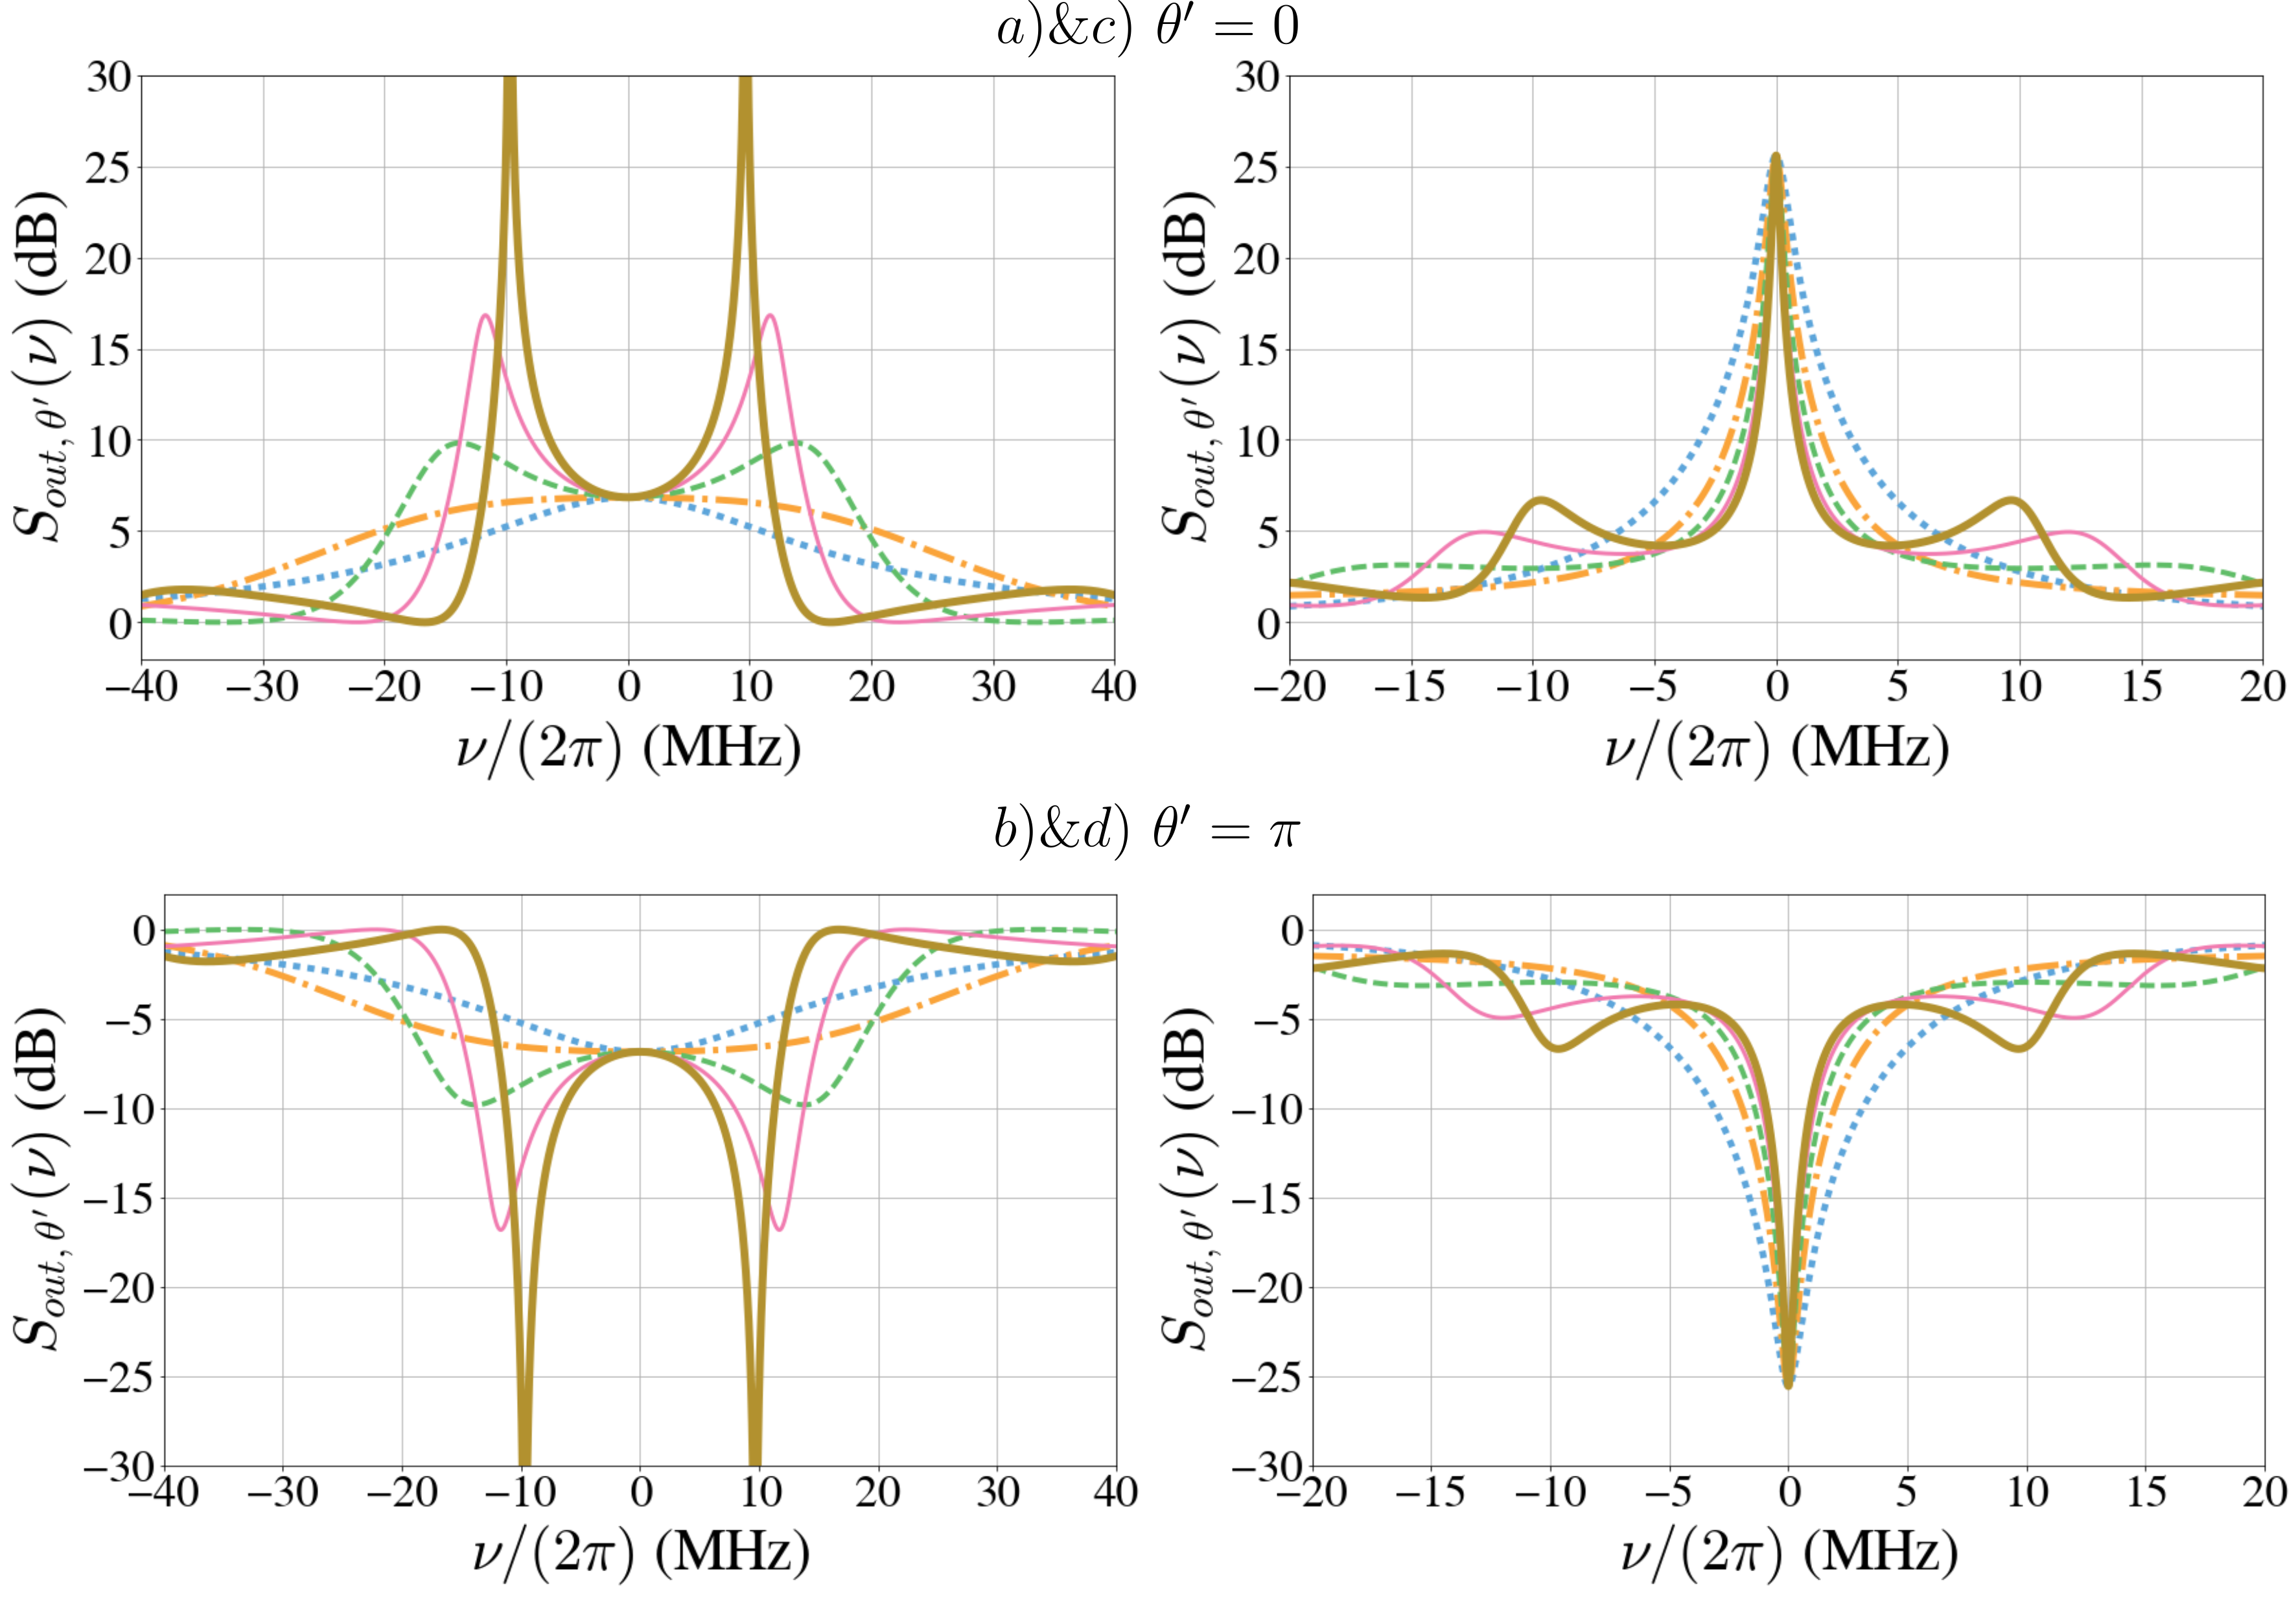
\includegraphics[width=.9\textwidth]{figure2.png}
\vglue -1 cm
\textit{\textbf{\caption{\linespread{1}\small{Schematic setup. The nonlinear crystal performing parametric down-conversion on the incoming photons is placed in a cavity. The output fields on the right hand side is directly coupled back into the input channels of the other side without performing any measurement. The longer length of the loops support a finite time-delay in the feedback loop ($\tau_{a,b}$) and phase shift ($\phi_{a,b}$). Losses are also incorporated in the feedback loop with a beam splitter model.}}\label{fig:setup}}}
%\vglue -.3 cm
\end{figure}

\begin{figure}[h!]
\centering
%\vglue -.2 cm
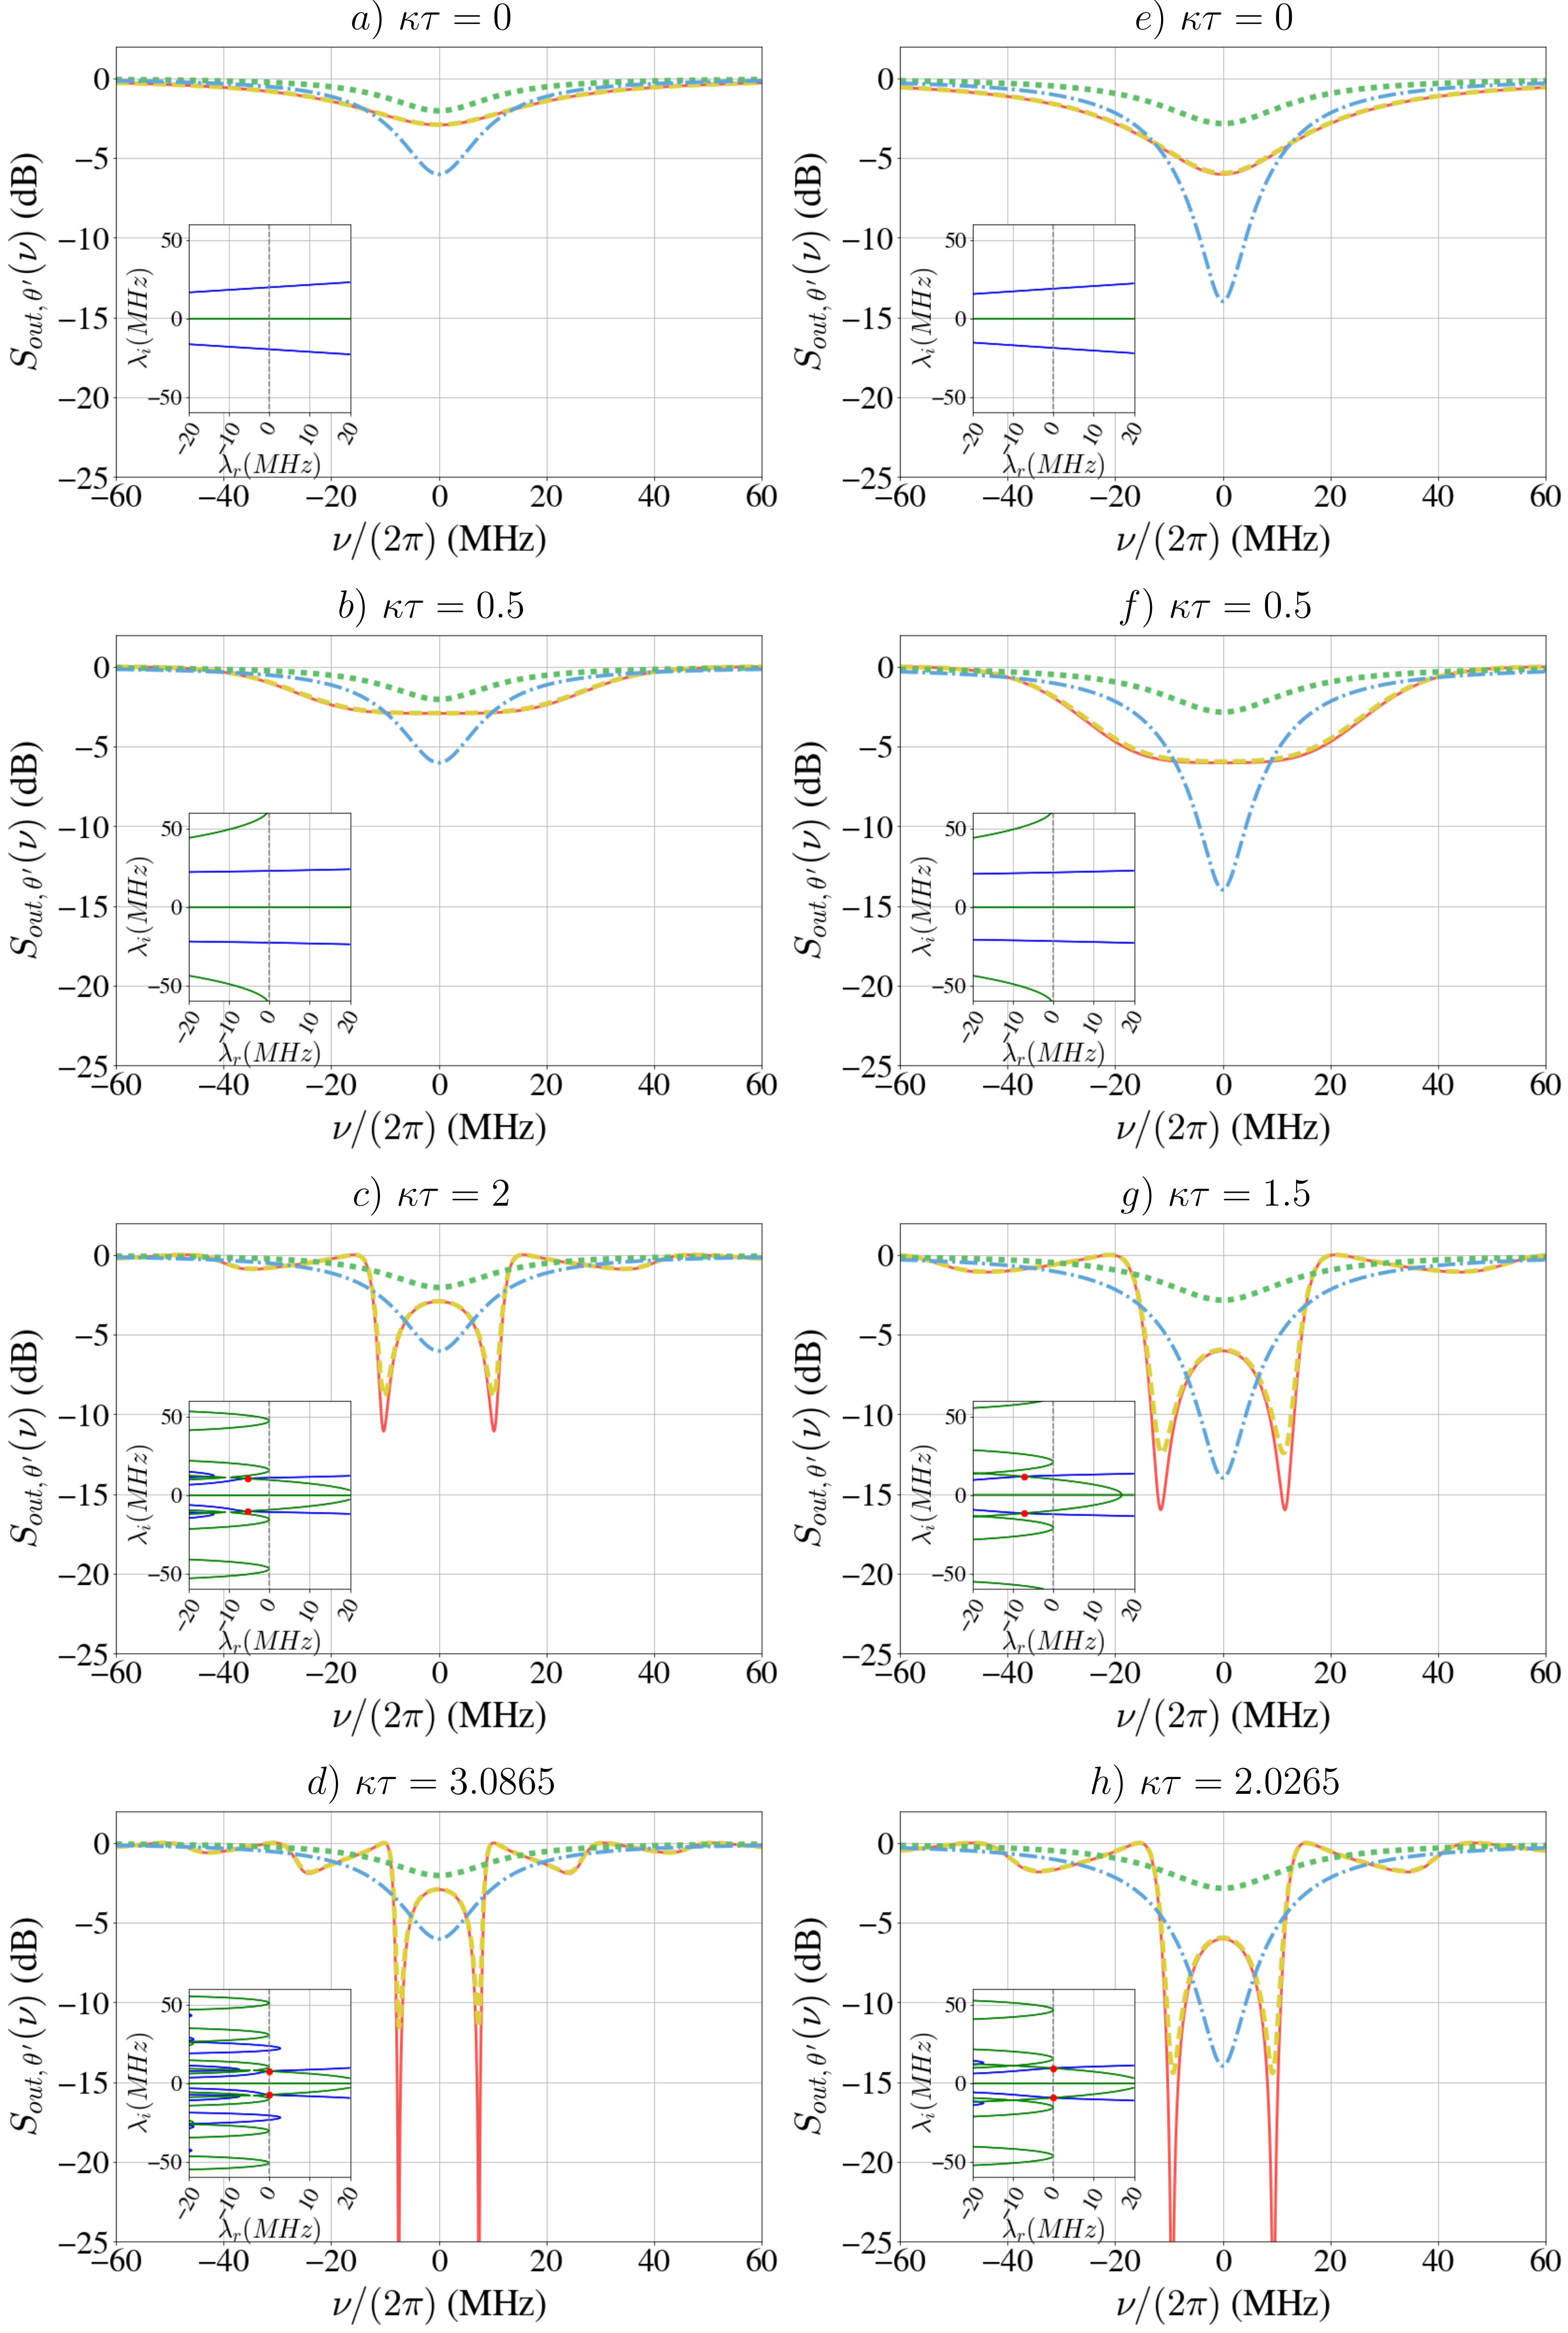
\includegraphics[width=.9\textwidth]{figure3.png}
\vglue -1 cm
\textit{\textbf{\caption{\linespread{1}\small{Schematic setup. The nonlinear crystal performing parametric down-conversion on the incoming photons is placed in a cavity. The output fields on the right hand side is directly coupled back into the input channels of the other side without performing any measurement. The longer length of the loops support a finite time-delay in the feedback loop ($\tau_{a,b}$) and phase shift ($\phi_{a,b}$). Losses are also incorporated in the feedback loop with a beam splitter model.}}\label{fig:setup}}}
%\vglue -.3 cm
\end{figure}

\begin{figure}[h!]
\centering
%\vglue -.2 cm
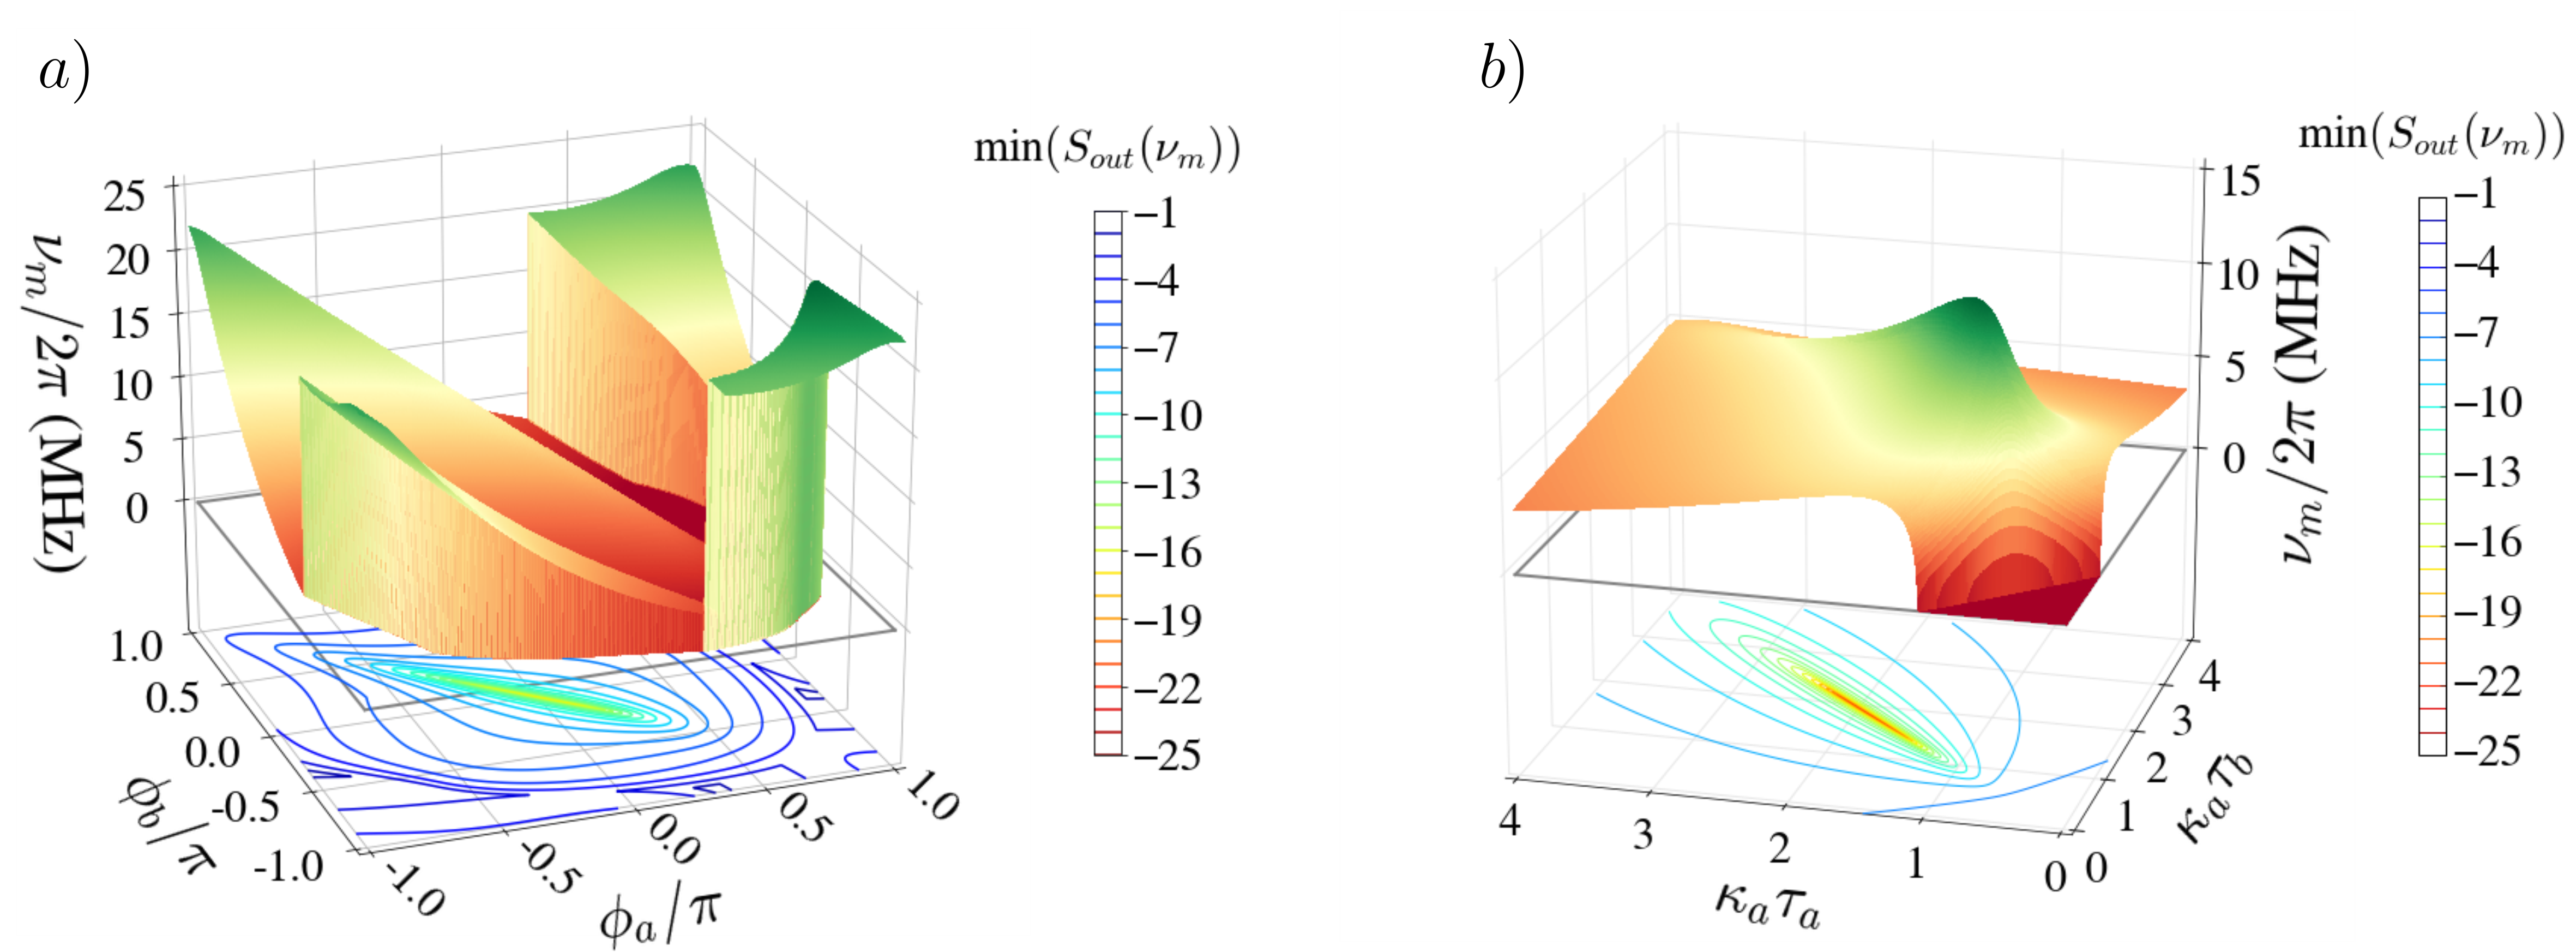
\includegraphics[width=.9\textwidth]{figure4.png}
\vglue -1 cm
\textit{\textbf{\caption{\linespread{1}\small{Schematic setup. The nonlinear crystal performing parametric down-conversion on the incoming photons is placed in a cavity. The output fields on the right hand side is directly coupled back into the input channels of the other side without performing any measurement. The longer length of the loops support a finite time-delay in the feedback loop ($\tau_{a,b}$) and phase shift ($\phi_{a,b}$). Losses are also incorporated in the feedback loop with a beam splitter model.}}\label{fig:setup}}}
%\vglue -.3 cm
\end{figure}

\section{Differences in the loops}

\section*{References}
\bibliographystyle{iopart-num}
\bibliography{NDPA}

\end{document}